\section{Results}
\label{sec:results}

\subsection{DSO4: the forecast beats the naive baseline}
LightGBM reduces the error on the daily total from 31.6\% (same day last week) to \textbf{25.3\%} wMAPE,
a 19.9\% relative improvement (RMSE 7.0 contacts per day), and it is also better than SARIMA (27.7\%) and
Prophet (35.9\%) on the total (Figure~\ref{fig:forecast}). Per family (Table~\ref{tab:forecast}), it wins on
the largest one (where is my order); SARIMA is slightly better on two small families and Prophet on one.
Small families have 1--3 contacts a day, so their error is dominated by Poisson noise; staffing is therefore
decided on the total. The most important features are the recent levels (28- and 7-day means, 31\% and 29\% of
the gain), the same-weekday mean (9\%), the days since the last major sale and the orders promised for the
coming days: the model uses the \emph{order drivers}, as intended. \textbf{Verdict: main idea kept.}

\begin{figure}[!htbp]
\centering
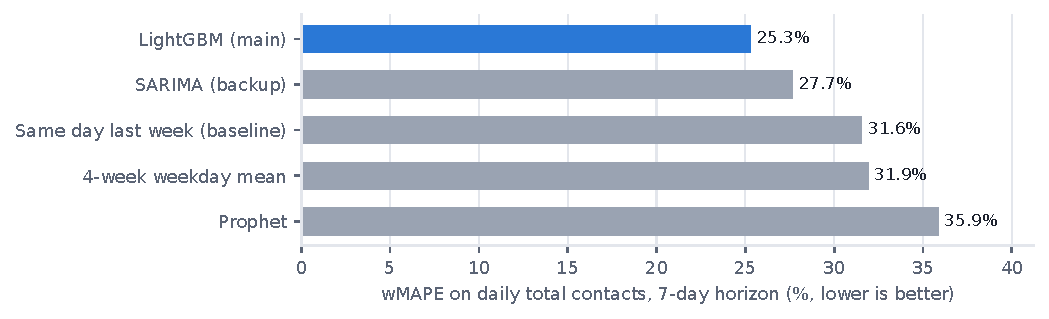
\includegraphics[width=0.86\textwidth]{figures/forecast_wmape.pdf}
\caption{Forecast error on the daily total (rolling backtest, 46 origins, 7-day horizon).}
\label{fig:forecast}
\end{figure}

\begin{table}[!htbp]
\centering\small
\caption{wMAPE (\%) per intent family; lower is better, best in bold.}
\label{tab:forecast}
\begin{tabular}{@{}lrrrrr@{}}
\toprule
\textbf{Family} & \textbf{LightGBM} & \textbf{Same day last week} & \textbf{4-week mean} & \textbf{SARIMA} &
\textbf{Prophet} \\
\midrule
Total & \textbf{25.3} & 31.6 & 31.9 & 27.7 & 35.9 \\
Where is my order & \textbf{36.9} & 45.5 & 48.8 & 42.3 & 52.1 \\
After delivery & 38.0 & 45.1 & 41.9 & \textbf{35.2} & 43.7 \\
Order admin & 54.7 & 68.0 & 55.9 & 53.7 & \textbf{52.7} \\
Cancel / refund & 83.8 & 102.9 & 86.1 & \textbf{81.3} & 90.5 \\
\bottomrule
\end{tabular}
\end{table}

\subsection{DSO4: the twin is faithful}
The twin passes all six fidelity checks (Table~\ref{tab:fidelity}). The first three prove that the engine is
correct (it reproduces Erlang C within 3\%); the last three show it is consistent with its inputs: daily volumes,
hourly profile and handle times are statistically indistinguishable from the history. \textbf{Verdict: kept.}

\begin{table}[!htbp]
\centering\small
\caption{Fidelity of the twin.}
\label{tab:fidelity}
\begin{tabular}{@{}llll@{}}
\toprule
\textbf{Check} & \textbf{Twin} & \textbf{Reference} & \textbf{Rule} \\
\midrule
Erlang C: probability of waiting & 0.279 & 0.285 (error 2.2\%) & error $<$ 5\% \\
Erlang C: mean wait & 33.3 s & 34.2 s (error 2.7\%) & error $<$ 5\% \\
Erlang C: answered within 20 s & 76.5\% & 75.9\% (error 0.8\%) & error $<$ 5\% \\
Daily volume vs history (4 weeks) & 491 / day & 488 / day, KS $p$ = 0.998 & $p > 0.05$ \\
Hour-of-day profile & --- & total variation distance 0.015 & $< 0.05$ \\
Handle time vs ticket logs & 273 s & 272 s, KS $p$ = 0.35 & $p > 0.05$ \\
\bottomrule
\end{tabular}
\end{table}

\subsection{BO4: testing a plan before a peak}
For each peak week we compare the plan a manager would build from the normal forecast (\emph{unprepared})
with the plan built after testing the scenario in the twin (\emph{prepared}), on the same customers. Preparing
always protects the service, and every difference is significant (Figure~\ref{fig:bo4}, Table~\ref{tab:bo4}):
understaffed hours fall by 60--84\%, abandonment by 55--78\%, and the mean wait of live customers by 60--82\%.
Preparing costs extra labour, so the money result depends on what a lost customer is worth. With our
assumption of €8, testing first saves \textbf{€6,991 net over the four peak weeks}; it loses €692 in the staff
shortage week, where the break-even value of a lost customer is €12. A repeat contact plus the risk of losing
the customer usually costs more than €6--12, which is why the break-even, not the euro figure, is the robust
result. Running 10 replications of a week takes 4.5--15.6 seconds, so a manager can test many options.

\begin{figure}[!htbp]
\centering
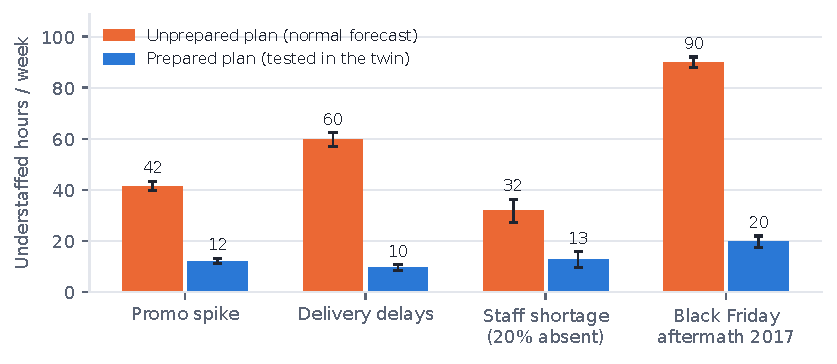
\includegraphics[width=0.86\textwidth]{figures/bo4_understaffed.pdf}
\caption{Understaffed hours per peak week, unprepared vs prepared plan (mean of 10 seeds, 95\% CI).}
\label{fig:bo4}
\end{figure}

\begin{table}[!htbp]
\centering\small
\caption{Testing first, per peak week (unprepared $\rightarrow$ prepared, 10 seeds). Net saving = avoided
lost-customer cost minus extra labour, with its 95\% CI.}
\label{tab:bo4}
\begin{tabularx}{\textwidth}{@{}Yllrr@{}}
\toprule
\textbf{Scenario} & \textbf{Answered $<$ 20 s} & \textbf{Abandonment} & \textbf{Net saving (€)} & \textbf{Break-even} \\
\midrule
Promo spike & 76.1\% $\rightarrow$ 91.9\% & 11.7\% $\rightarrow$ 4.5\% & +226 [129; 323] & €7.4 \\
Delivery delays & 67.8\% $\rightarrow$ 93.7\% & 15.5\% $\rightarrow$ 3.8\% & +1,196 [935; 1,458] & €6.2 \\
Staff shortage (20\% absent) & 81.6\% $\rightarrow$ 92.6\% & 9.8\% $\rightarrow$ 4.4\% & $-$692 [$-$987; $-$397] & €12.1 \\
Black Friday aftermath 2017 & 45.0\% $\rightarrow$ 87.2\% & 29.0\% $\rightarrow$ 6.4\% & +6,261 [5,985; 6,538] & €3.0 \\
\bottomrule
\end{tabularx}
\end{table}

\subsection{DSO3: CP-SAT planning}
In a normal week the CP-SAT plan costs \textbf{€7,050}, against €11,760 for a schedule sized for the busiest
hour (\textbf{$-$40\%}), and still answers 92.4\% of chats within 20 s, above the 80\% target, with every labour
rule respected (Figure~\ref{fig:dso3}). The cost per handled contact falls from €3.20 to €1.95. The rule-based
backup (Erlang C with two shift templates) saves 17\%. In the promotion week, CP-SAT costs €9,762 against
€16,464 (\textbf{$-$41\%}) at 91.9\% service. \textbf{Verdict: main idea kept} ($\geq$5\% cheaper at the target).
A fixed schedule \emph{tuned by hand} to the right level costs about the same in a normal week, because the
Olist hourly profile is flat from 10:00 to 22:00; CP-SAT's value is that it finds this level automatically for
every week and scenario, guarantees the requirement hour by hour and the labour rules, and adapts when demand
has peaks.

\begin{figure}[!htbp]
\centering
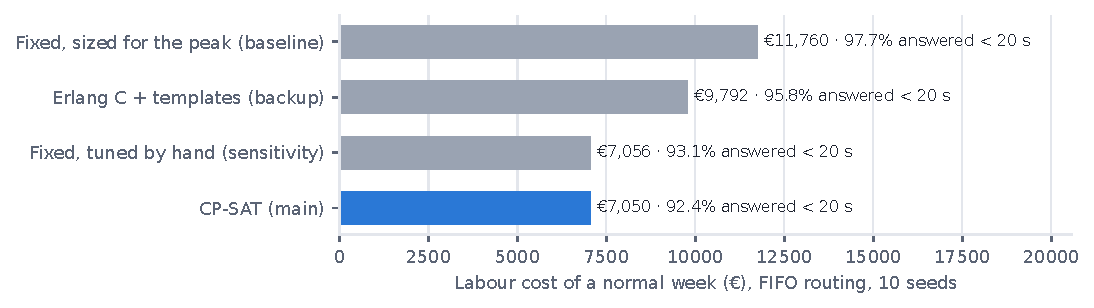
\includegraphics[width=0.86\textwidth]{figures/dso3_planners.pdf}
\caption{Weekly labour cost of the four planners in a normal week, with the service level each one reaches.}
\label{fig:dso3}
\end{figure}

\subsection{DSO1: routing}
On \textbf{unseen stressed days}, both routers beat FIFO significantly (Table~\ref{tab:dso1}): PPO cuts the speed
of answer by \textbf{13.9\%} and raises the service level by 3.4 points; the tuned skill score cuts the mean wait
of live customers by 11.6\% and abandonment by 7.2\%. In the \textbf{full peak weeks} the picture changes
(Figure~\ref{fig:dso1}): neither router changes the mean wait significantly; both reduce abandonment
significantly (skill score $-$6.5\% to $-$9.6\%, PPO $-$3.7\% to $-$4.5\%), and PPO cuts the
90th-percentile wait by 18--25\%. PPO serves customers who have waited long or are about to leave: a fairness
gain that the mean hides. Peak weeks differ from the training days (a backlog that carries over several days,
planned overtime), and PPO was trained on single days.
\textbf{Verdict (switch rule): not met}: the $\geq$10\% gain does not hold in peak weeks. The tuned skill score
is the production candidate (robust, explainable), and PPO stays the research track.

\begin{table}[!htbp]
\centering\small
\caption{Routing on 20 unseen stressed days (40 paired runs). In brackets: change vs FIFO; all significant.}
\label{tab:dso1}
\setlength{\tabcolsep}{4pt}
\begin{tabular}{@{}lllll@{}}
\toprule
\textbf{Router} & \textbf{ASA} & \textbf{Mean wait (all live)} & \textbf{$<$ 20 s} & \textbf{Abandonment} \\
\midrule
FIFO + skill matching (baseline) & 25.2 s & 37.5 s & 59.7\% & 19.7\% \\
Tuned skill score (backup) & 22.6 s ($-$10.3\%) & 33.1 s ($-$11.6\%) & 62.2\% & 18.3\% ($-$7.2\%) \\
MaskablePPO (main) & 21.7 s ($-$13.9\%) & 35.4 s ($-$5.6\%) & 63.0\% & 18.8\% ($-$4.6\%) \\
\bottomrule
\end{tabular}
\end{table}

\begin{figure}[!htbp]
\centering
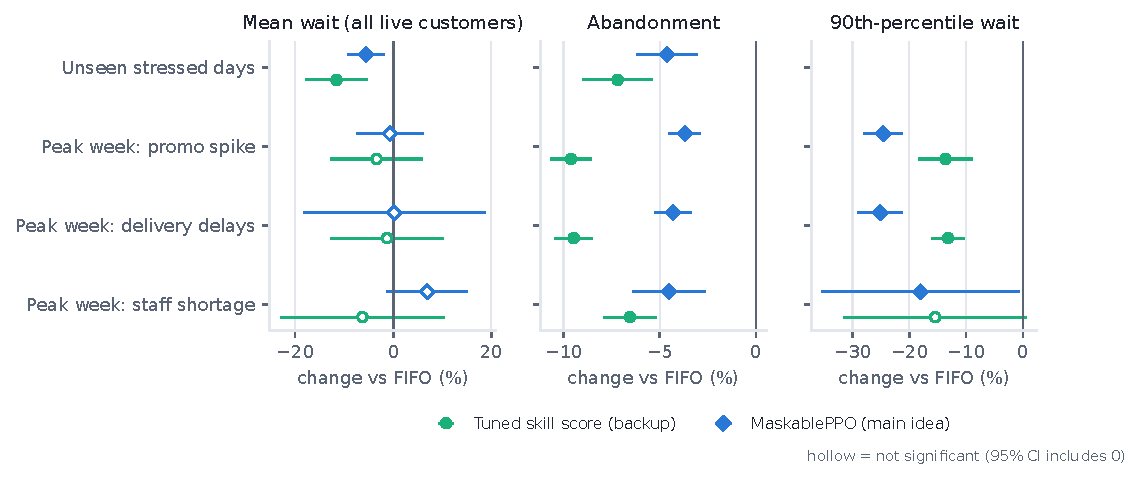
\includegraphics[width=0.98\textwidth]{figures/dso1_routing.pdf}
\caption{Change vs FIFO with 95\% CI. Filled markers are significant; hollow ones are not (the 90th-percentile
wait was not measured in the stressed-day study).}
\label{fig:dso1}
\end{figure}

\subsection{DSO2: retrieval, answers and the judge}
\textbf{Retrieval.} On 255 questions, bge-m3 + FAISS finds the right policy section first 80.0\% of the time and in
the top 4 \textbf{96.9\%} of the time, against 52.9\% and 80.4\% for keyword search (Figure~\ref{fig:retrieval}).
The gap is largest in French (34 questions: 94\% vs 15\% at rank 1), because the embeddings are multilingual.
\textbf{Verdict: retrieval beats the baseline.}

\begin{figure}[!htbp]
\centering
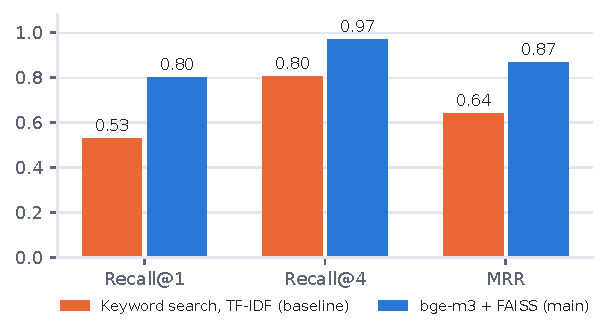
\includegraphics[width=0.62\textwidth]{figures/dso2_retrieval.pdf}
\caption{Retrieval on 255 Bitext questions (17 intents).}
\label{fig:retrieval}
\end{figure}

\textbf{Answers.} Table~\ref{tab:dso2} compares the variants on the same 12 customers. This paired batch was run
on 19--20 October with our first local models (Qwen2.5-3B advisor and client, Llama-3.2-3B judge); the template
variant was later re-run on 40 customers.
The pure RAG advisor writes well-grounded answers (faithfulness 0.99), but nothing in them can be
\emph{verified} as the policy action, and the judge accepted none of them. The hybrid, where the rules engine
decides and the LLM writes, gives a checkable action that is right in \textbf{12/12} chats and the best customer
satisfaction (\textbf{4.33/5}); in 4 of the 12 chats a safety net replaced an LLM draft by the approved text.
Tool calls worked 100\% of the time once tool gating was in place (48\% before).

\begin{table}[!htbp]
\centering\small
\caption{Advisor variants (BO2 KPIs). ``Verified'' compares the advisor's action with the rules' action; the
template variant is judged by the checklist, the LLM variants by the LLM judge.}
\label{tab:dso2}
\setlength{\tabcolsep}{4pt}
\begin{tabular}{@{}lrrrrrr@{}}
\toprule
\textbf{Variant} & \textbf{Chats} & \textbf{Verified} & \textbf{Judge: correct} & \textbf{CSAT} &
\textbf{Faithful.} & \textbf{Similarity} \\
\midrule
Template (backup) & 40 & 100\% & 100\% & 3.83 & 0.65 & 1.00 \\
Pure RAG (idea A) & 12 & not verifiable & 0\% & 3.58 & 0.99 & 0.74 \\
RAG + rules engine (hybrid) & 12 & \textbf{100\%} & 17\% & \textbf{4.33} & 0.70 & 0.79 \\
\bottomrule
\end{tabular}
\end{table}

\textbf{The judge.} Against labels on 60 historical chats, neither judge reaches the 0.4 kappa needed to be
trusted (Table~\ref{tab:judge}). The 3B LLM judge is close to chance; the checklist is better on resolution
(kappa 0.39, Spearman 0.50). Two reasons: a 3B judge is too weak (it called policy-correct answers ``invented
promises''), and the labels are proxies (a generator's answer key), so the satisfaction labels are partly
random. \textbf{Verdict: the AI reviewer is not trusted yet}; the deterministic action check is the
production quality signal, and the judge is advisory.

\begin{table}[!htbp]
\centering\small
\caption{Judge calibration: quadratic weighted kappa on 60 chats (trusted from 0.4).}
\label{tab:judge}
\begin{tabular}{@{}lrrr@{}}
\toprule
\textbf{Judge} & \textbf{Satisfaction} & \textbf{Resolution} & \textbf{Within $\pm$1 point} \\
\midrule
LLM judge (Llama-3.2-3B) & 0.06 & 0.06 & 58--65\% \\
Checklist reviewer (backup) & 0.07 & \textbf{0.39} & 63--65\% \\
\bottomrule
\end{tabular}
\end{table}

\textbf{Tool calling.} Making the LLM choose tools taught us more than any score. SmolLM3-3B never emitted a real
tool call on its own (0 of 186 traced advisor calls); it even \emph{narrated} fake calls (``I've called
lookup\_order...'') with invented facts. Forcing a tool call at the investigation step (the reply is pre-started
with the tool-call marker) gave 6 of 6 real calls with the right order id. The hosted Nemotron models call tools
correctly in about 1.5 s. On the client side, the customer's \code{view\_my\_order\_page} tool caught a wrong
``delivered'' claim by the advisor in a trial.

\subsection{Monitoring the AI components}
\label{sec:monitoring}
Over the 1,339 traced LLM calls and 219 saved chats (live and evaluation, all periods), the monitoring page
(Figure~\ref{fig:monitoringpage}) gives a sober picture (Figures~\ref{fig:latency} and~\ref{fig:confidence}):

\begin{figure}[!htbp]
\centering
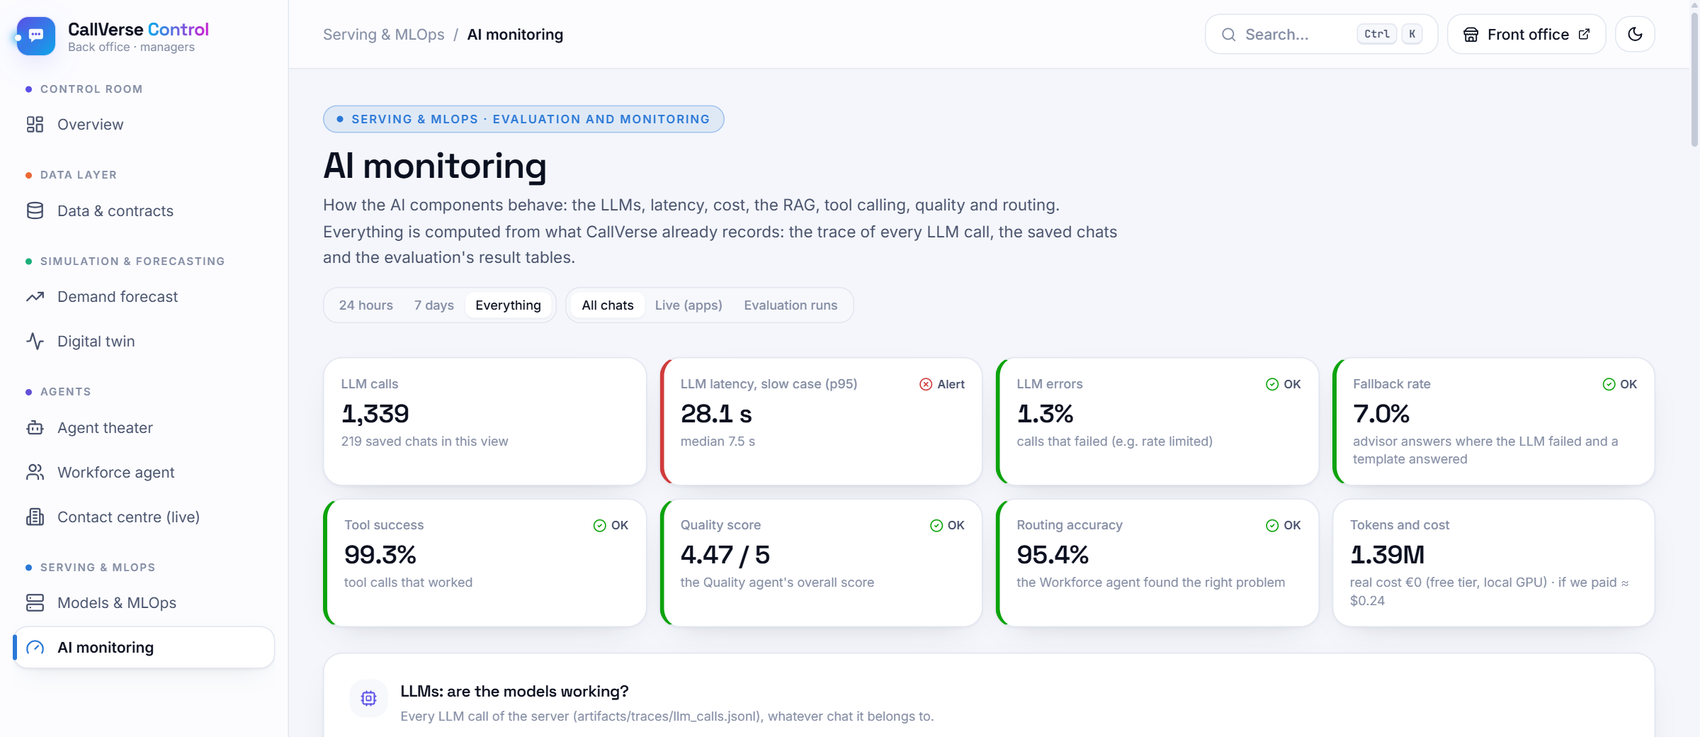
\includegraphics[width=\textwidth]{figures/screen_monitoring.png}
\caption{The AI monitoring page of the back office (all periods, all chats). Each headline indicator turns
amber or red past its threshold, always with an icon and a word (OK, Watch, Alert) as well as a colour.}
\label{fig:monitoringpage}
\end{figure}

\begin{itemize}
  \item \textbf{Latency.} The p95 latency is 28 s (red), but it comes from the local-GPU period: the local
        SmolLM3 advisor answers in 16.2 s at the median (p95 43.1 s), the hosted Nemotron 3.5 Super advisor in
        2.0 s (p95 8.0 s). This measurement drove the switch to OpenRouter.
  \item \textbf{Fallbacks and tools.} 7.0\% of the advisor's LLM answers fell back to a template (amber threshold:
        20\%), and 99.3\% of the tool calls succeeded. Of the tool calls whose caller is recorded, 132 were made by
        fixed pipeline steps and only 13 were chosen by the LLM: the system is honest ``workflow plus agent'', not
        a fully autonomous agent.
  \item \textbf{Routing.} The Workforce agent found the right problem in 95.4\% of the chats; its confidence can
        be trusted: 99.5\% right when it is above 0.9 (186 chats), 78\% between 0.5 and 0.7. The main confusion is
        \code{track\_order} vs \code{track\_delivery} (6 chats), two close intents of the same family (where is my order).
  \item \textbf{Judge vs customer.} The judge's score and the customer's CSAT correlate only weakly (Pearson 0.21),
        another sign that the judge is not yet a reliable proxy.
  \item \textbf{Cost.} The real cost is €0 (free tier and local GPU). At the reference price, the 1.39 million
        tokens would cost \$0.24, about \$0.0002 per resolved chat; 90.9\% of the chats were resolved.
\end{itemize}

\begin{figure}[!htbp]
\centering
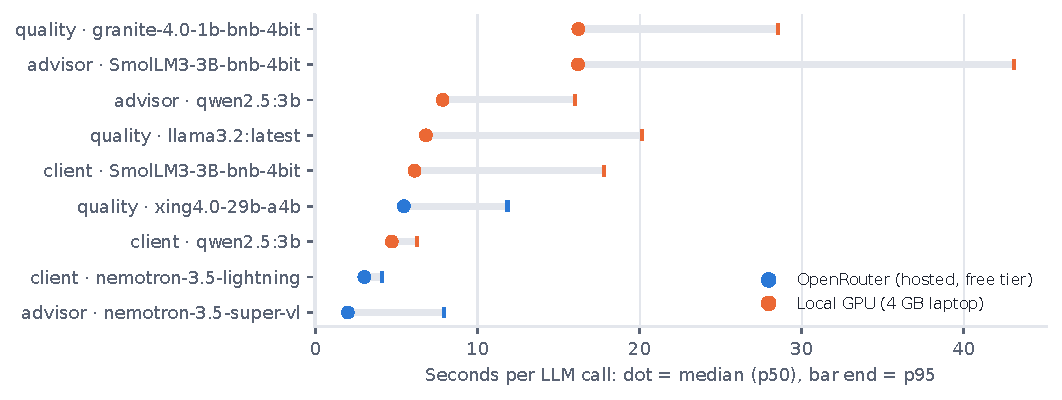
\includegraphics[width=0.86\textwidth]{figures/llm_latency.pdf}
\caption{Latency per LLM call by agent and model (models with at least 10 calls).}
\label{fig:latency}
\end{figure}

\begin{figure}[!htbp]
\centering
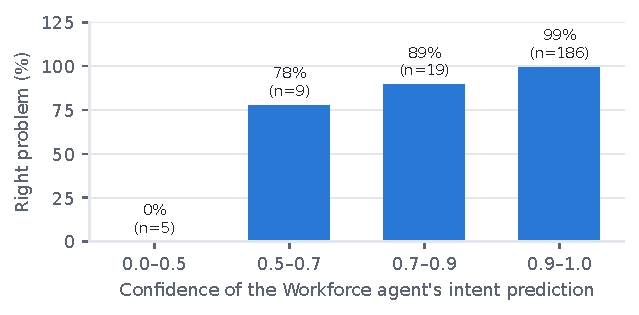
\includegraphics[width=0.6\textwidth]{figures/routing_confidence.pdf}
\caption{Routing accuracy by confidence of the intent prediction (219 chats).}
\label{fig:confidence}
\end{figure}

\subsection{Scorecard}
Table~\ref{tab:scorecard} applies the switch rules. The foundation (DSO4) and the planning objective (DSO3) pass
clearly. DSO1 and DSO2 bring measurable gains, but our own rules put the backup or a hybrid in production.

\begin{table}[!htbp]
\centering\small
\caption{BO/DSO scorecard (\code{artifacts/evaluations/scorecard.json}).}
\label{tab:scorecard}
\begin{tabularx}{\textwidth}{@{}lYcY@{}}
\toprule
\textbf{DSO} & \textbf{Result} & \textbf{Rule met} & \textbf{In production} \\
\midrule
DSO1 routing & PPO: ASA $-$13.9\% on stressed days; in peak weeks mean wait not significant, abandonment
  $-$4\% & no & Tuned skill score \\
DSO2 advisor + judge & Recall@4 96.9\%; hybrid 12/12 verified actions, CSAT 4.33; judge kappa $<$ 0.4 & no &
  Hybrid advisor; template backup; checklist reviewer \\
DSO3 planning & Labour cost $-$40\% at 92.4\% service; labour rules respected & yes & CP-SAT \\
DSO4 forecast + twin & wMAPE 25.3\% vs 31.6\%; all fidelity checks pass; €6,991 net saved over 4 peak weeks &
  yes & LightGBM + twin \\
\bottomrule
\end{tabularx}
\end{table}
